% ============================================================
% 数电实验报告 — 实验四：基于硬件描述语言电路设计
% ============================================================

\documentclass[12pt]{ctexart}

% --- 宏包 ---
\usepackage{graphicx}
\usepackage{amsmath}
\usepackage{xcolor}
\usepackage{float}
\usepackage{booktabs}
\usepackage{siunitx}
\usepackage{fancyhdr}
\usepackage{caption}
\usepackage{subcaption}
\usepackage{hyperref}
\usepackage{makecell}
\usepackage{enumitem}
\usepackage[outputdir=build]{minted}

\sisetup{per-mode=symbol}

\graphicspath{{./figures/}{../figures/}}

\usepackage[left=2.5cm, right=2.5cm, top=2.5cm, bottom=2.5cm]{geometry}

\setlength{\jot}{6pt}
\setlength{\headheight}{15pt}
\linespread{1.5}
\setlist{nosep}

% --- VHDL 代码样式 ---
\setminted[vhdl]{
    fontsize=\small,
    frame=single,
    linenos,
    breaklines,
    tabsize=4,
    numbersep=8pt,
    xleftmargin=2em
}

% --- 页眉页脚 ---
\pagestyle{fancy}
\fancyhead[C]{数字电子技术实验}
\fancyfoot[C]{\thepage}

\begin{document}

% ==================== 封面 ====================
\thispagestyle{empty}

\begin{figure}[t]
    \centering
    
\includegraphics[width=13cm]{logo1.png}
\end{figure}

\vspace*{\fill}
    \begin{center}
        \Huge\textbf{数字电子技术基础}

        \vspace{0.3cm}
        \Huge\textbf{实验报告}

        \vspace{1cm}
        \LARGE\textbf{实验四：基于硬件描述语言电路设计}
    \end{center}
\vspace*{\fill}

\begin{table}[H]
    \centering
    \large
    \begin{tabular}{ll}
    \toprule
    \textbf{课程:} & 数字电子技术实验 \\
    \textbf{组员1:} & 郭浩然 2024303980 \\
    \textbf{组员2:} & 庞铭洋 2024302539 \\
    \textbf{组号:} & 15 \\
    \textbf{时间:} & \today \\
    \bottomrule
    \end{tabular}
\end{table}

\newpage

% ==================== 正文 ====================

\section{实验目的}

\begin{enumerate}
    \item 掌握 VHDL 硬件描述语言的基本语法，理解实体（Entity）、结构体（Architecture）、信号（Signal）和进程（Process）等核心概念。
    \item 学习使用 VHDL 分别设计组合逻辑电路（异或门、七段码译码器）和时序逻辑电路（计数器、分频器），并在 Quartus II 中进行编译和波形仿真验证。
    \item 掌握 Quartus II 中 VHDL 文件的编译、生成原理图模块符号（Create Symbol Files）以及在顶层原理图中调用 VHDL 模块的基本流程。
    \item 能够将多个独立设计的 VHDL 模块在顶层原理图中组合连接，实现较复杂的数字系统设计，并下载到 DE0 开发板进行硬件验证。
\end{enumerate}

\section{实验要求}

\begin{enumerate}
    \item \textbf{要求 1}：学习并掌握硬件描述语言 VHDL，熟悉门电路的逻辑功能，并用硬件描述语言实现门电路的设计。参考"参考内容 1"中给出的与门源程序，编写一个异或门逻辑电路。用 Quartus II 波形仿真验证，下载到 DE0 开发板验证。
    \item \textbf{要求 2}：熟悉中规模器件译码器的逻辑功能，用硬件描述语言实现其设计。参考"参考内容 2"中给出的将 8421BCD 码转换成 0--9 的七段码译码器源程序，编写一个将二进制码转换成 0--E 的七段码译码器。用 Quartus II 波形仿真验证，下载到 DE0 开发板，利用开发板上的数码管验证。
    \item \textbf{要求 3}：熟悉时序电路计数器的逻辑功能，用硬件描述语言实现其设计。参考"参考内容 3"中给出的四位二进制计数器的源程序，编写一个计数器实现 0--E 计数。用 Quartus II 波形仿真验证。
    \item \textbf{要求 4}：熟悉分频电路的逻辑功能，并用硬件描述语言实现其设计。参考"参考内容 4"中给出的 50M 分频器的源程序，编写一个能实现占空比 50\% 的 5M 和 50M 分频器即两个输出，输出信号频率分别为 10Hz 和 1Hz。下载到 DE0 开发板验证（提示：利用 DE0 板上已有的 50M 晶振作为输入信号，通过开发板上两个的 LED 灯观察输出信号）。
    \item \textbf{要求 5}：利用已经实现的 VHDL 模块文件，顶层文件采用原理图设计方法，实现 A 学号后 4 位（3980）、F,E,E,L、学号后 4 位（0938）共 12 位字符在七段数码管上自动循环显示，频率 1Hz 和 10Hz 可以自动切换（提示：如何将 VHDL 模块文件在顶层原理图文件中引用，参考参考内容 5）。
\end{enumerate}

\section{实验设备}

\begin{itemize}
    \item Quartus II 开发软件
    \item DE0 开发板（FPGA 型号：Cyclone V 5CEBA4F23C7）
    \item USB-Blaster 下载线及计算机
    \item 七段数码管显示模块及相关输入、输出引脚
\end{itemize}

\section{实验原理}

\subsection{VHDL 基本结构}

VHDL（Very High Speed Integrated Circuit Hardware Description Language）是一种用于描述数字电路行为和结构的硬件描述语言。一个完整的 VHDL 设计文件由三部分组成：

\begin{enumerate}
    \item \textbf{库引用}：通过 \texttt{library} 和 \texttt{use} 语句引入标准库。\texttt{ieee.std\_logic\_1164.all} 提供 \texttt{std\_logic} 和 \texttt{std\_logic\_vector} 等标准逻辑类型；\texttt{ieee.numeric\_std.all} 提供 \texttt{unsigned}、\texttt{signed} 等数值类型及算术运算支持。
    \item \textbf{实体（Entity）}：定义模块的外部接口，通过 \texttt{port()} 声明输入输出端口。端口类型包括 \texttt{std\_logic}（单比特信号）和 \texttt{std\_logic\_vector}（多比特总线），方向有 \texttt{in}、\texttt{out}、\texttt{inout} 和 \texttt{buffer}。
    \item \textbf{结构体（Architecture）}：描述模块的内部行为或结构。可使用并发信号赋值语句实现组合逻辑，或使用 \texttt{process} 进程块实现时序逻辑。
\end{enumerate}

\subsection{组合逻辑设计}

组合逻辑电路的输出仅取决于当前输入，无记忆功能。在 VHDL 中，组合逻辑可通过以下两种方式实现：

\begin{itemize}
    \item \textbf{并发信号赋值}：直接在结构体中使用赋值语句，如 \texttt{C <= A xor B;}，描述异或门逻辑。
    \item \textbf{进程中的 \texttt{case} 语句}：在 \texttt{process} 块中使用 \texttt{case} 语句进行多路选择，适用于译码器等多输入多输出的组合逻辑。
\end{itemize}

七段码译码器是典型的组合逻辑电路：根据 4 位 BCD 输入，通过 \texttt{case} 语句选择对应的 7 位段选码输出。DE0 开发板的七段数码管为共阳极结构，段选信号低电平有效（0 表示点亮，1 表示熄灭）。各数字对应的段选编码如表~\ref{tab:hex_decode} 所示。

\begin{table}[H]
    \centering
    \caption{8421BCD 转七段码译码真值表}
    \label{tab:hex_decode}
    \begin{tabular}{cccc}
        \toprule
        \textbf{BCD 输入} & \textbf{十六进制} & \textbf{seg\_out[6:0]} & \textbf{显示字符} \\
        \midrule
        0000 & 0 & 1000000 & 0 \\
        0001 & 1 & 1111001 & 1 \\
        0010 & 2 & 0100100 & 2 \\
        0011 & 3 & 0110000 & 3 \\
        0100 & 4 & 0011001 & 4 \\
        0101 & 5 & 0010010 & 5 \\
        0110 & 6 & 0000010 & 6 \\
        0111 & 7 & 1111000 & 7 \\
        1000 & 8 & 0000000 & 8 \\
        1001 & 9 & 0010000 & 9 \\
        1010 & A & 0001000 & A \\
        1011 & b & 0000011 & b \\
        1100 & C & 1000110 & C \\
        1101 & d & 0100001 & d \\
        1110 & E & 0000110 & E \\
        1111 & -- & 1111111 & 灭灯 \\
        \bottomrule
    \end{tabular}
\end{table}

\subsection{时序逻辑设计}

时序逻辑电路的输出不仅与当前输入有关，还与电路的历史状态有关，依赖时钟信号驱动状态变化。在 VHDL 中，时序逻辑通过 \texttt{process(clk, rst)} 进程块实现，使用 \texttt{rising\_edge(clk)} 检测时钟上升沿来触发寄存器更新。

模 $N$ 计数器是最基本的时序逻辑电路之一。以模 15 计数器为例，每个时钟上升沿计数值加 1，当计数到 14（即十六进制 E）后，下一个时钟回到 0，同时产生一个时钟周期宽度的进位脉冲 COUT。计数器还具有异步清零功能：当复位信号 \texttt{rst} 为低电平时，计数值立即清零。

\subsection{分频器原理}

分频器通过对高频时钟信号进行计数来产生低频输出信号。若输入时钟频率为 $f_{\text{clk}}$，期望输出频率为 $f_{\text{out}}$，则需要的半周期计数值为
\[
    N = \frac{f_{\text{clk}}}{2 \times f_{\text{out}}}
\]
计数器每计满 $N$ 次，将输出信号翻转一次，即可产生占空比 50\% 的方波。

对于 DE0 开发板上 50MHz 的晶振时钟：
\begin{itemize}
    \item 分频到 1Hz：$N = 50{,}000{,}000 / 2 = 25{,}000{,}000$
    \item 分频到 10Hz：$N = 50{,}000{,}000 / (2 \times 10) = 2{,}500{,}000$
\end{itemize}

\subsection{综合设计原理}

要求 5 的综合设计需要将计数器、译码器和分频/速度切换模块组合，实现 12 位字符的循环显示，并在 1Hz 和 10Hz 之间自动切换速度。

显示序列为 \texttt{2539FEEL3980}，由三部分组成：组员 B 学号后 4 位（2539）、固定字符 F,E,E,L、以及组员 A 学号后 4 位（3980）。M12 计数器从 0 计数到 11，每个计数值通过特殊七段码译码器映射到对应的显示字符，如表~\ref{tab:display_map} 所示。

\begin{table}[H]
    \centering
    \caption{综合设计显示序列映射表}
    \label{tab:display_map}
    \begin{tabular}{cccc}
        \toprule
        \textbf{计数值} & \textbf{BCD 码} & \textbf{显示字符} & \textbf{SG\_OUT[6:0]} \\
        \midrule
        0  & 0000 & 2 & 0100100 \\
        1  & 0001 & 5 & 0010010 \\
        2  & 0010 & 3 & 0110000 \\
        3  & 0011 & 9 & 0010000 \\
        4  & 0100 & F & 0001110 \\
        5  & 0101 & E & 0000110 \\
        6  & 0110 & E & 0000110 \\
        7  & 0111 & L & 1000111 \\
        8  & 1000 & 3 & 0110000 \\
        9  & 1001 & 9 & 0010000 \\
        10 & 1010 & 8 & 0000000 \\
        11 & 1011 & 0 & 1000000 \\
        \bottomrule
    \end{tabular}
\end{table}

综合设计由三个核心模块组成：

\begin{enumerate}
    \item \textbf{M12 计数器}（\texttt{exa4\_3\_2}）：0 到 11 循环计数，带使能信号 \texttt{en}，仅在 \texttt{en=1} 时计数加 1。计数到 11 后回到 0，同时输出一个 \texttt{cout} 脉冲，表示一轮显示结束。
    \item \textbf{特殊七段码译码器}（\texttt{exa4\_2\_2}）：根据 M12 计数器的当前值，输出对应字符的七段码。
    \item \textbf{自动切换控制器}（\texttt{exa4\_auto\_1hz\_10hz}）：内部集成 1Hz 和 10Hz 两种分频模式。每当 M12 计数器完成一轮显示（\texttt{cout=1}），自动切换到另一种速度。其 \texttt{tick} 输出作为 M12 计数器的使能输入，形成闭环控制。
\end{enumerate}

顶层原理图中三个模块的连接关系为：50MHz 时钟同时连接到自动切换控制器和 M12 计数器的时钟端；复位信号同时连接到两者的复位端；自动切换控制器的 \texttt{tick} 输出连接到 M12 计数器的 \texttt{en} 输入；M12 计数器的 \texttt{dout} 连接到译码器的 \texttt{BCD\_IN}；M12 计数器的 \texttt{cout} 反馈连接到自动切换控制器的 \texttt{loop\_end} 输入；译码器的 \texttt{SG\_OUT} 输出连接到 HEX0 数码管引脚。

\section{实验内容}

\subsection{要求 1：异或门电路}

\subsubsection{创建工程与编写 VHDL}

打开 Quartus II，选择 \textbf{File $\rightarrow$ New Project Wizard} 新建工程。器件选择 DE0 开发板对应的 Cyclone V \texttt{5CEBA4F23C7}。选择 \textbf{File $\rightarrow$ New $\rightarrow$ VHDL File} 新建 VHDL 文件，输入异或门源码并保存为 \texttt{exa4\_1\_xor.vhd}。

\begin{minted}{vhdl}
library ieee;
use ieee.std_logic_1164.all;

entity exa4_1_xor is
port(
    A : in  std_logic;
    B : in  std_logic;
    C : out std_logic
);
end exa4_1_xor;

architecture rtl of exa4_1_xor is
begin
    C <= A xor B;
end rtl;
\end{minted}
\captionof{listing}{异或门 VHDL 源码（exa4\_1\_xor.vhd）}
\label{lst:xor}

该设计定义了一个具有两个输入端 A、B 和一个输出端 C 的异或门，结构体中使用并发信号赋值语句直接描述异或逻辑。

\subsubsection{编译与生成原理图框图}

点击 \textbf{Start Compilation} 对 VHDL 文件进行完整编译。编译通过后，选择 \textbf{File $\rightarrow$ Create/Update $\rightarrow$ Create Symbol Files for Current File}，将 VHDL 模块生成可在原理图中调用的模块符号文件（\texttt{.bsf}）。

\subsubsection{建立顶层原理图}

选择 \textbf{File $\rightarrow$ New $\rightarrow$ Block Diagram/Schematic File} 新建原理图文件。在元件库的 Project 目录下找到刚生成的 \texttt{exa4\_1\_xor} 符号并放置到原理图中，然后添加输入引脚 A、B 和输出引脚 C，完成连线。顶层原理图如图~\ref{fig:task1_circuit} 所示。

\begin{figure}[H]
    \centering
    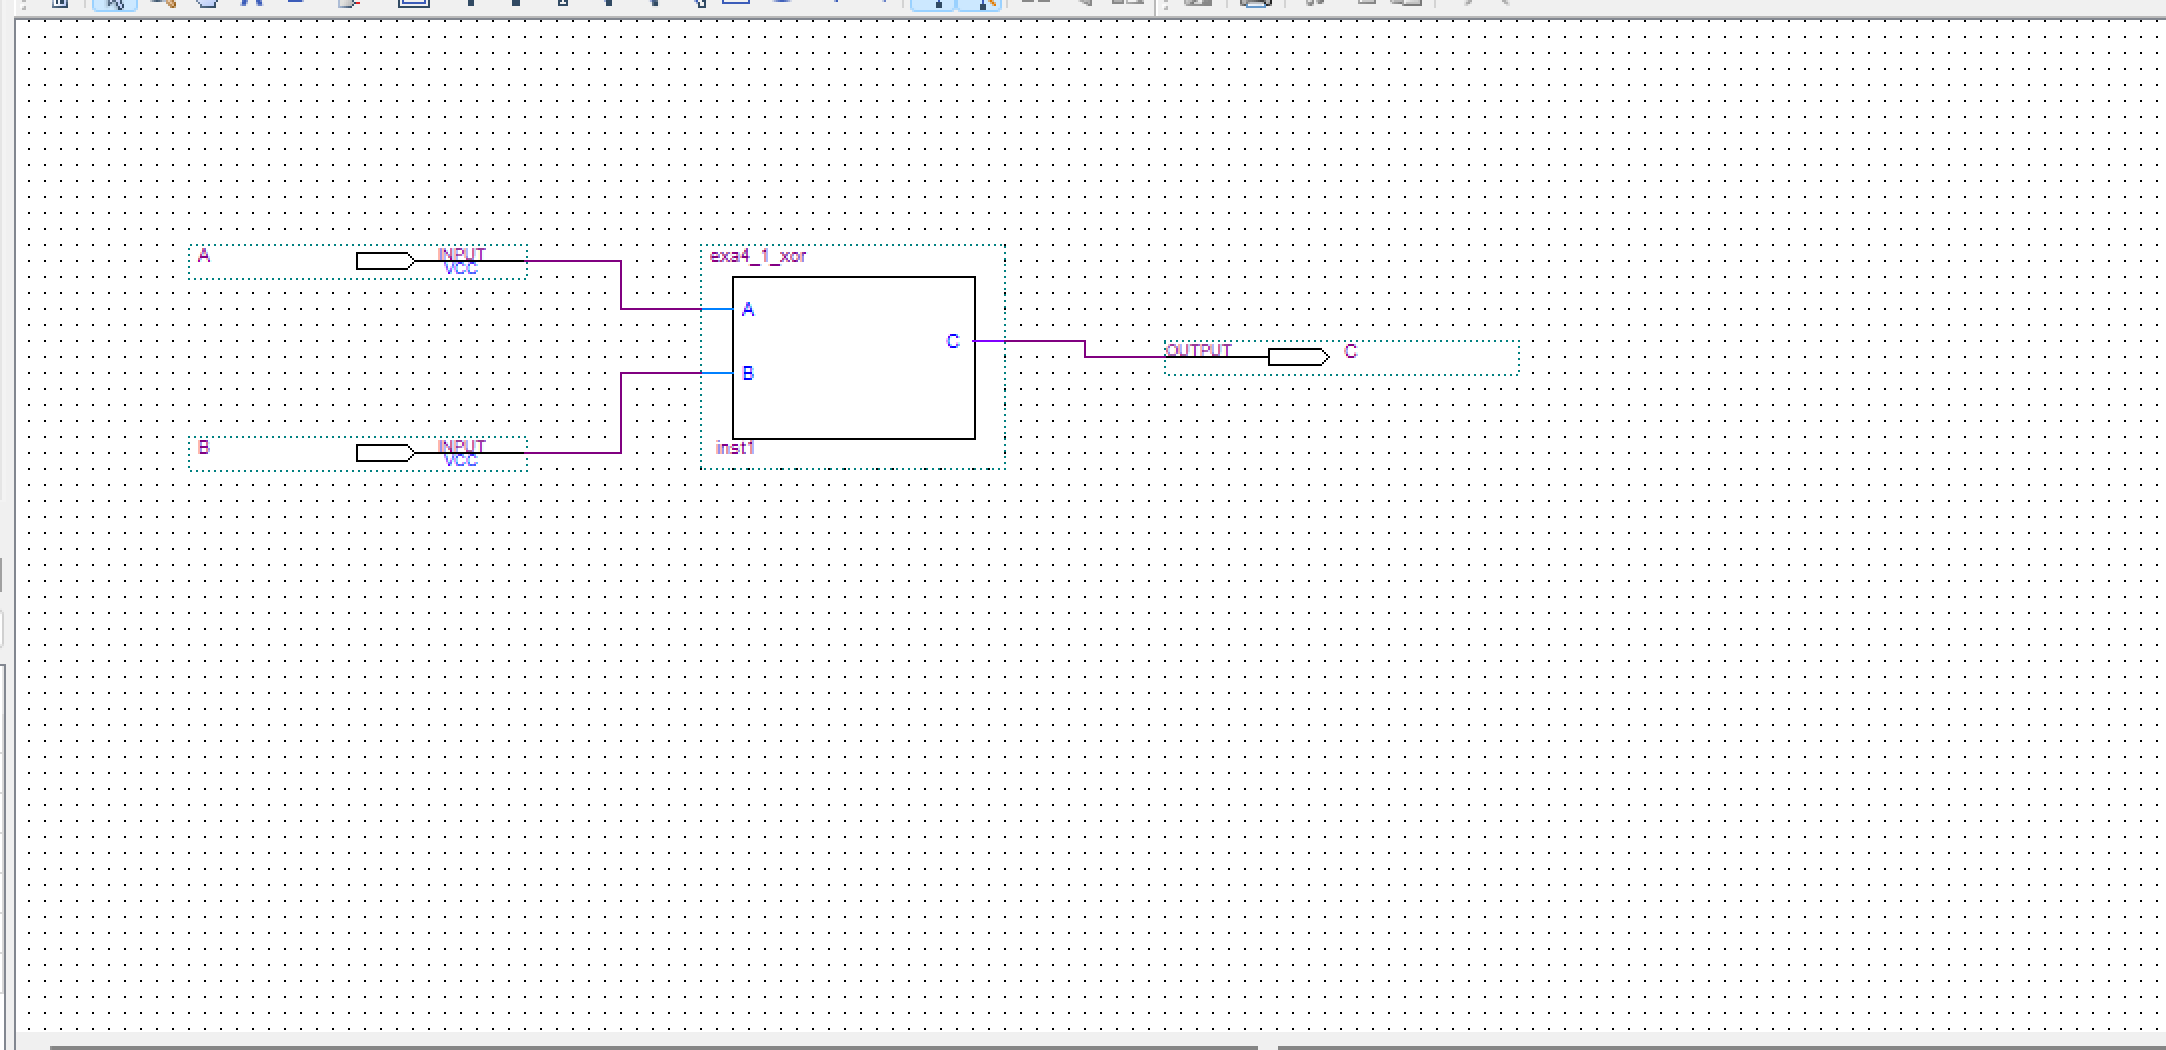
\includegraphics[width=0.85\textwidth]{要求1电路.png}
    \caption{要求 1 异或门 BDF 原理图}
    \label{fig:task1_circuit}
\end{figure}

\subsubsection{波形仿真验证}

将原理图文件设置为顶层实体并重新编译。选择 \textbf{File $\rightarrow$ New $\rightarrow$ Vector Waveform File} 新建波形文件，加入 A、B、C 三个信号。设置 A 的周期为 20ns、B 的周期为 40ns，运行功能仿真。仿真结果如图~\ref{fig:task1_sim} 所示。

\begin{figure}[H]
    \centering
    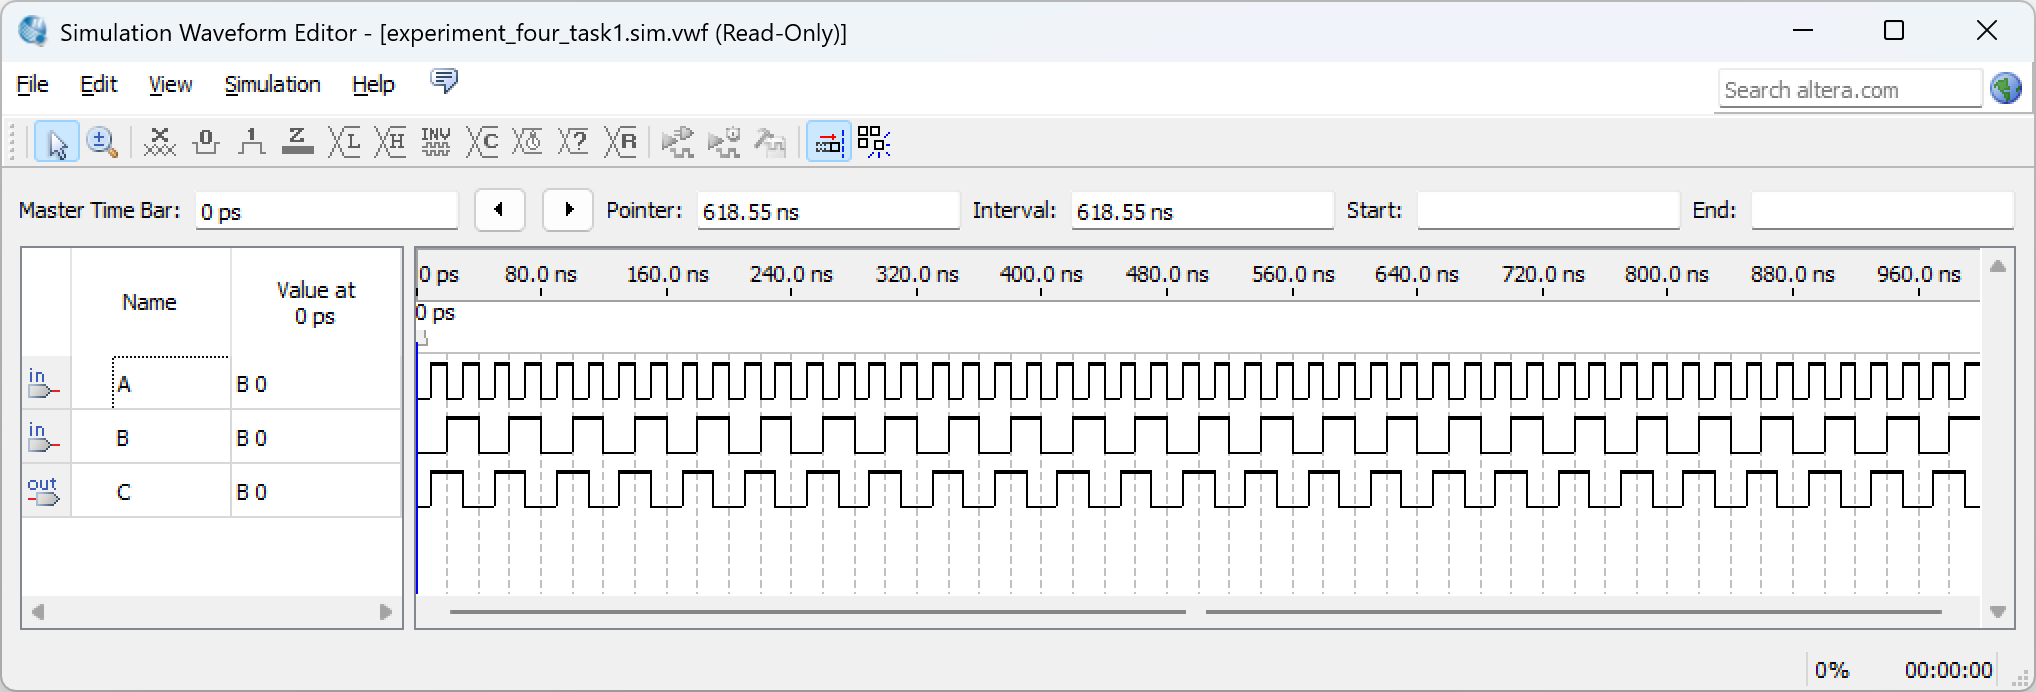
\includegraphics[width=0.95\textwidth]{要求1仿真.png}
    \caption{要求 1 异或门仿真波形}
    \label{fig:task1_sim}
\end{figure}

从仿真波形可以看出，当 A 和 B 的输入电平相同时，输出 C 为低电平；当 A 和 B 的输入电平不同时，输出 C 为高电平，符合异或门的逻辑功能。

\subsubsection{引脚分配与下载验证}

打开 Pin Planner，将输入 A、B 分别分配到开发板的拨动开关 SW0（PIN\_U13）和 SW1（PIN\_V13），输出 C 分配到 LEDR0（PIN\_AA2）。重新编译工程后，连接 USB-Blaster，选择 JTAG 模式下载 \texttt{.sof} 文件到 FPGA。在开发板上拨动开关，观察 LED 指示灯正确反映异或逻辑。

\subsection{要求 2：8421BCD 转七段码译码器}

\subsubsection{创建工程与编写 VHDL}

新建 Quartus II 工程，创建 VHDL 文件 \texttt{exa4\_2\_hex\_0e.vhd}，编写支持 0--E 共 15 个字符显示的七段码译码器。

\begin{minted}{vhdl}
library ieee;
use ieee.std_logic_1164.all;

entity exa4_2_hex_0e is
port(
    data_in : in  std_logic_vector(3 downto 0);
    seg_out : out std_logic_vector(6 downto 0)
);
end exa4_2_hex_0e;

architecture rtl of exa4_2_hex_0e is
begin
    process(data_in)
    begin
        case data_in is
            when "0000" => seg_out <= "1000000"; -- 0
            when "0001" => seg_out <= "1111001"; -- 1
            when "0010" => seg_out <= "0100100"; -- 2
            when "0011" => seg_out <= "0110000"; -- 3
            when "0100" => seg_out <= "0011001"; -- 4
            when "0101" => seg_out <= "0010010"; -- 5
            when "0110" => seg_out <= "0000010"; -- 6
            when "0111" => seg_out <= "1111000"; -- 7
            when "1000" => seg_out <= "0000000"; -- 8
            when "1001" => seg_out <= "0010000"; -- 9
            when "1010" => seg_out <= "0001000"; -- A
            when "1011" => seg_out <= "0000011"; -- b
            when "1100" => seg_out <= "1000110"; -- C
            when "1101" => seg_out <= "0100001"; -- d
            when "1110" => seg_out <= "0000110"; -- E
            when others => seg_out <= "1111111"; -- blank
        end case;
    end process;
end rtl;
\end{minted}
\captionof{listing}{七段码译码器 VHDL 源码（exa4\_2\_hex\_0e.vhd）}
\label{lst:hex}

该译码器将 4 位 BCD 输入转换为 7 位段选信号输出。\texttt{process} 的敏感列表为 \texttt{data\_in}，当输入变化时自动重新计算输出，实现纯组合逻辑行为。段选码已按共阳极低电平有效编码，可直接驱动 DE0 开发板的七段数码管。

\subsubsection{编译、生成原理图框图与建立顶层原理图}

编译 VHDL 文件后生成模块符号。新建 BDF 原理图，放置 \texttt{exa4\_2\_hex\_0e} 符号，添加 4 位输入总线 \texttt{data\_in[3..0]} 和 7 位输出总线 \texttt{seg\_out[6..0]}，完成连线。顶层原理图如图~\ref{fig:task2_circuit} 所示。

\begin{figure}[H]
    \centering
    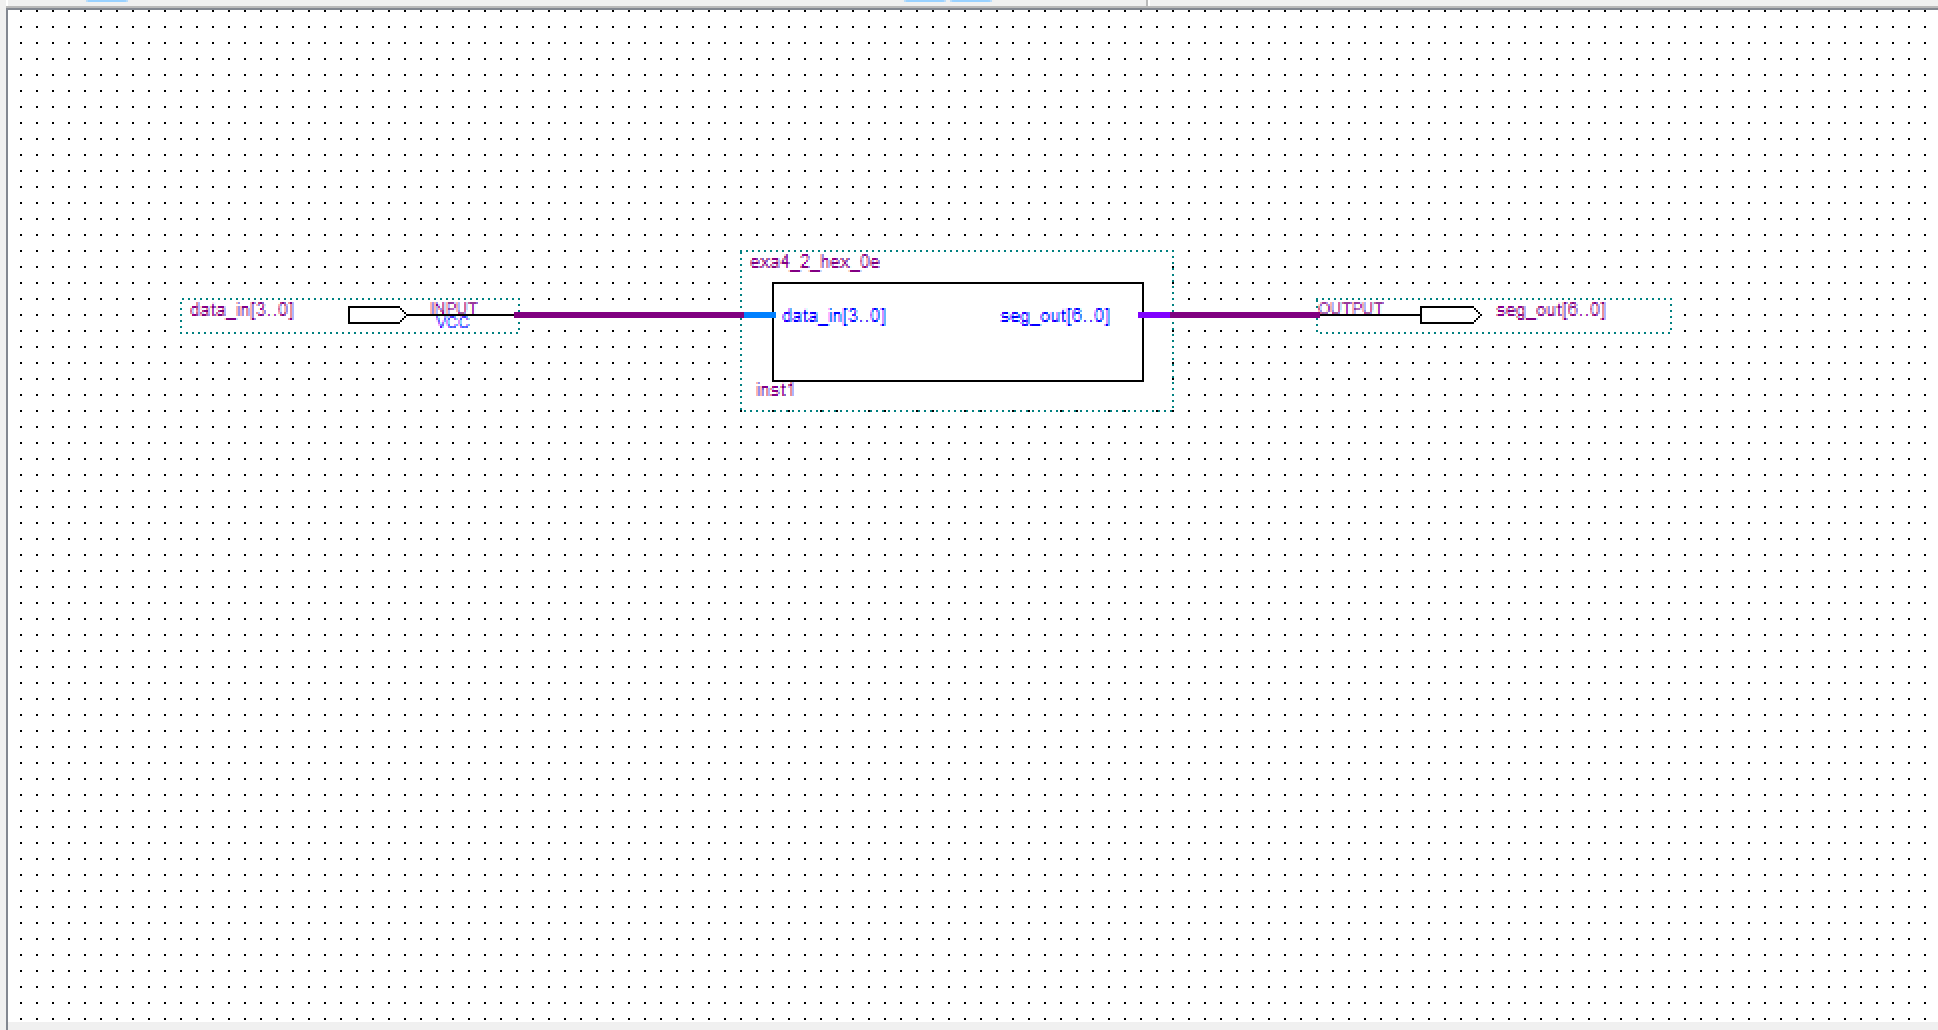
\includegraphics[width=0.85\textwidth]{要求2电路.png}
    \caption{要求 2 七段码译码器 BDF 原理图}
    \label{fig:task2_circuit}
\end{figure}

\subsubsection{波形仿真验证}

建立波形文件，设置 \texttt{data\_in} 依次从 0000 变化到 1111，每个输入保持一定时间。运行仿真后，检查 \texttt{seg\_out} 的输出是否与表~\ref{tab:hex_decode} 中的真值表一致。仿真结果表明，16 种输入组合的段选输出均正确。

\subsubsection{引脚分配与下载验证}

将 \texttt{data\_in[3:0]} 分配到拨动开关 SW3--SW0（PIN\_T12、PIN\_T13、PIN\_V13、PIN\_U13），\texttt{seg\_out[6:0]} 分配到 HEX0 数码管的 7 个段选引脚（PIN\_AA22、PIN\_Y21、PIN\_Y22、PIN\_W21、PIN\_W22、PIN\_V21、PIN\_U21）。重新编译并下载到 FPGA 后，拨动开关选择不同的 BCD 码，观察数码管正确显示 0--E 各字符。

\subsection{要求 3：模 15 计数器}

\subsubsection{创建工程与编写 VHDL}

新建工程，创建 VHDL 文件 \texttt{exa4\_3\_counter\_0e.vhd}，编写模 15 计数器。

\begin{minted}{vhdl}
library ieee;
use ieee.std_logic_1164.all;
use ieee.numeric_std.all;

entity exa4_3_counter_0e is
port(
    clk  : in  std_logic;
    rst  : in  std_logic;
    DOUT : out std_logic_vector(3 downto 0);
    COUT : out std_logic
);
end exa4_3_counter_0e;

architecture rtl of exa4_3_counter_0e is
    signal count_q : unsigned(3 downto 0) := (others => '0');
    signal cout_q  : std_logic := '0';
begin
    process(clk, rst)
    begin
        if rst = '0' then
            count_q <= (others => '0');
            cout_q <= '0';
        elsif rising_edge(clk) then
            if count_q = to_unsigned(14, 4) then
                count_q <= (others => '0');
                cout_q <= '1';
            else
                count_q <= count_q + 1;
                cout_q <= '0';
            end if;
        end if;
    end process;

    DOUT <= std_logic_vector(count_q);
    COUT <= cout_q;
end rtl;
\end{minted}
\captionof{listing}{模 15 计数器 VHDL 源码（exa4\_3\_counter\_0e.vhd）}
\label{lst:counter}

该计数器使用 \texttt{ieee.numeric\_std} 库的 \texttt{unsigned} 类型进行计数，支持异步低电平复位。每个时钟上升沿计数加 1，当计数到 14 时下一个时钟回到 0 并产生一个周期的进位脉冲 COUT。

\subsubsection{编译、生成原理图框图与建立顶层原理图}

编译后生成模块符号。在顶层 BDF 中放置 \texttt{exa4\_3\_counter\_0e} 符号，连接时钟和复位输入、计数输出和进位输出。引脚分配如表~\ref{tab:task3_pins} 所示，顶层原理图如图~\ref{fig:task3_circuit} 所示。

\begin{table}[H]
    \centering
    \caption{要求 3 引脚分配表}
    \label{tab:task3_pins}
    \begin{tabular}{ccc}
        \toprule
        \textbf{端口名} & \textbf{引脚} & \textbf{对应硬件} \\
        \midrule
        clk     & PIN\_M9  & 50MHz 时钟 \\
        rst     & PIN\_U7  & KEY0 \\
        DOUT[3] & PIN\_Y3  & LEDR3 \\
        DOUT[2] & PIN\_W2  & LEDR2 \\
        DOUT[1] & PIN\_AA1 & LEDR1 \\
        DOUT[0] & PIN\_AA2 & LEDR0 \\
        COUT    & PIN\_N2  & LEDR4 \\
        \bottomrule
    \end{tabular}
\end{table}

\begin{figure}[H]
    \centering
    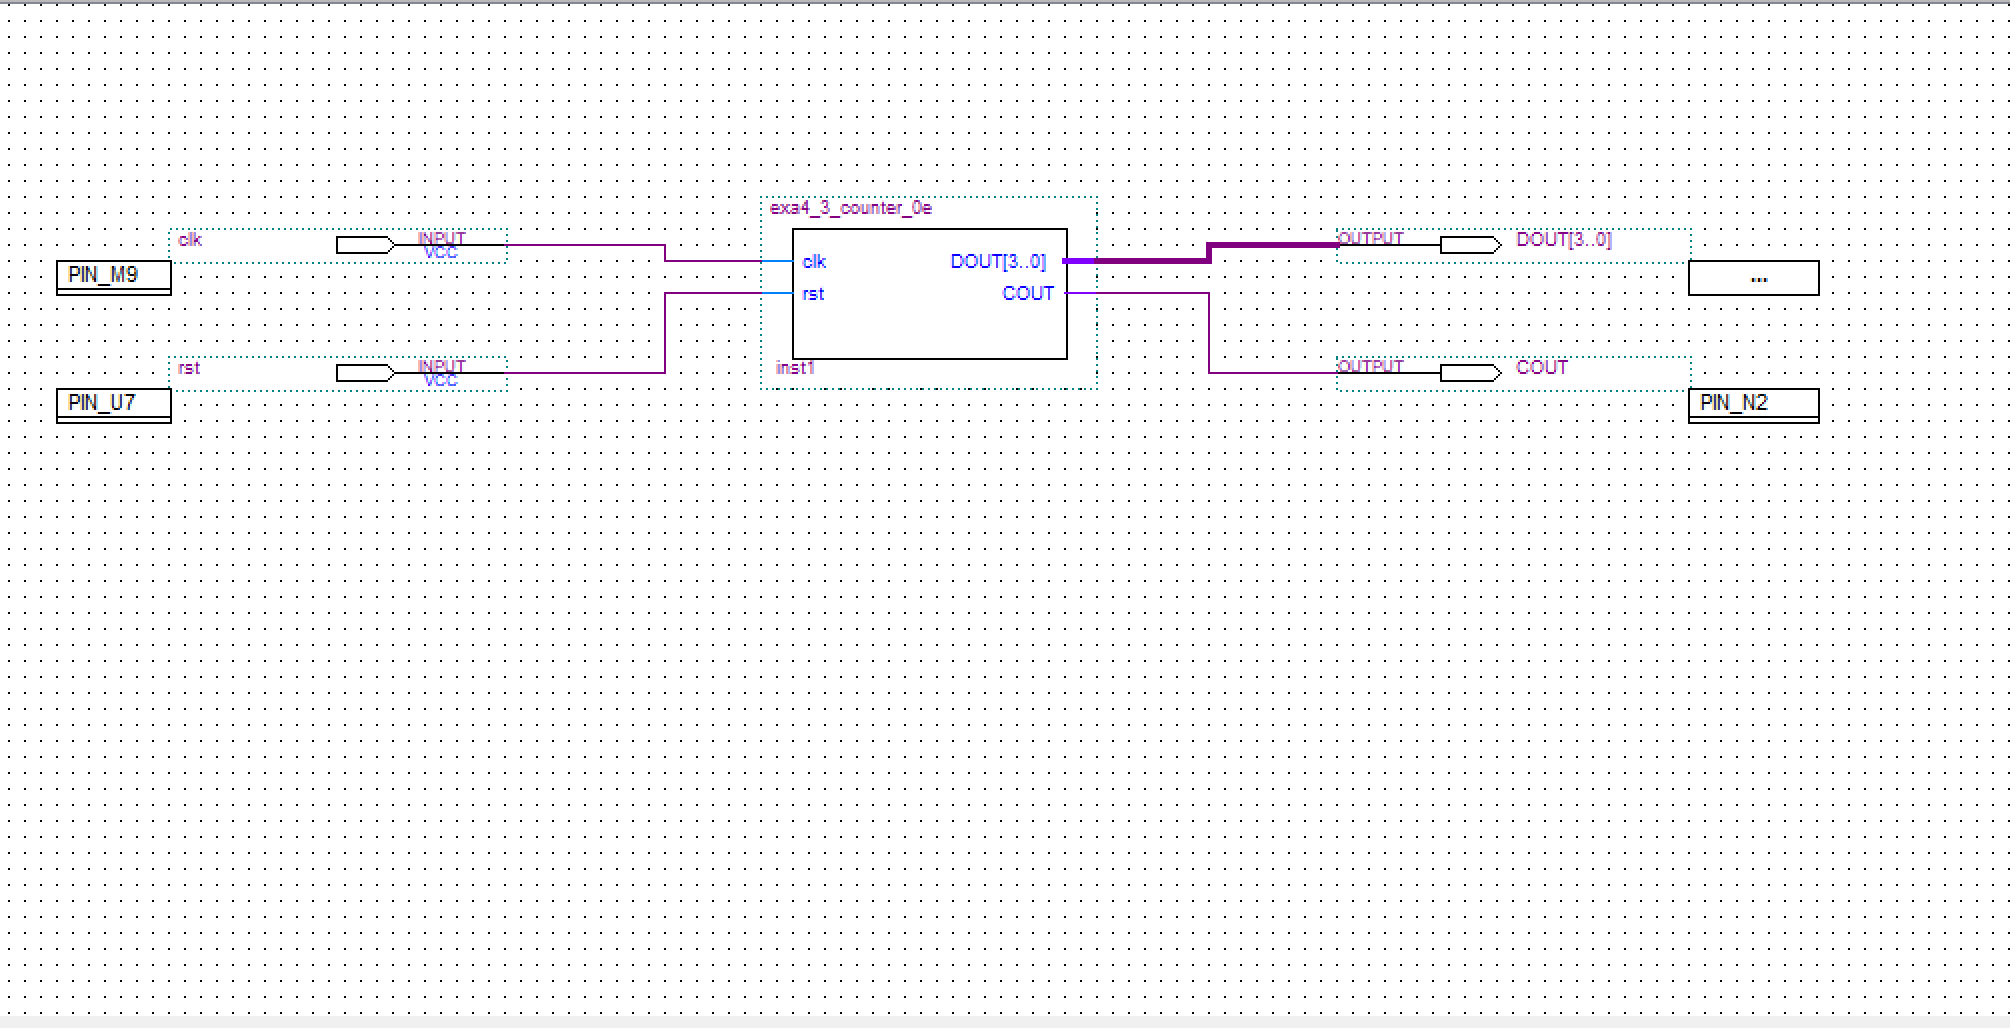
\includegraphics[width=0.85\textwidth]{要求3电路.png}
    \caption{要求 3 模 15 计数器 BDF 原理图}
    \label{fig:task3_circuit}
\end{figure}

\subsubsection{波形仿真验证}

建立波形文件，设置时钟信号周期，在仿真开始时给复位端一个短暂的低电平脉冲。运行仿真后，观察 DOUT 依次输出 0, 1, 2, \ldots, 14, 0, 1, \ldots 的循环计数序列，COUT 在每次计数从 14 回到 0 时产生一个高电平脉冲，验证了计数器功能正确。

\subsection{要求 4：50M 分频器}

\subsubsection{创建工程与编写 VHDL}

新建工程，创建 VHDL 文件 \texttt{exa4\_4\_divider\_1hz\_10hz.vhd}，编写同时输出 1Hz 和 10Hz 的双路分频器。

\begin{minted}{vhdl}
library ieee;
use ieee.std_logic_1164.all;

entity exa4_4_divider_1hz_10hz is
generic(
    HALF_PERIOD_1HZ  : positive := 25000000;
    HALF_PERIOD_10HZ : positive := 2500000
);
port(
    clk50    : in  std_logic;
    clk_1hz  : out std_logic;
    clk_10hz : out std_logic
);
end exa4_4_divider_1hz_10hz;

architecture rtl of exa4_4_divider_1hz_10hz is
    signal cnt_1hz  : integer range 0 to HALF_PERIOD_1HZ - 1 := 0;
    signal cnt_10hz : integer range 0 to HALF_PERIOD_10HZ - 1 := 0;
    signal out_1hz  : std_logic := '0';
    signal out_10hz : std_logic := '0';
begin
    process(clk50)
    begin
        if rising_edge(clk50) then
            if cnt_1hz = HALF_PERIOD_1HZ - 1 then
                cnt_1hz <= 0;
                out_1hz <= not out_1hz;
            else
                cnt_1hz <= cnt_1hz + 1;
            end if;

            if cnt_10hz = HALF_PERIOD_10HZ - 1 then
                cnt_10hz <= 0;
                out_10hz <= not out_10hz;
            else
                cnt_10hz <= cnt_10hz + 1;
            end if;
        end if;
    end process;

    clk_1hz <= out_1hz;
    clk_10hz <= out_10hz;
end rtl;
\end{minted}
\captionof{listing}{双路分频器 VHDL 源码（exa4\_4\_divider\_1hz\_10hz.vhd）}
\label{lst:divider}

分频器使用 \texttt{generic} 参数定义半周期计数值，使设计具有通用性。两路分频器共享同一个 \texttt{process}，各自独立计数。当计数达到半周期值时，输出信号翻转并重置计数，产生占空比 50\% 的方波。

\subsubsection{编译、生成原理图框图与建立顶层原理图}

编译后生成模块符号。在顶层 BDF 中放置分频器符号，连接输入时钟和两路输出。引脚分配如表~\ref{tab:task4_pins} 所示，顶层原理图如图~\ref{fig:task4_circuit} 所示。

\begin{table}[H]
    \centering
    \caption{要求 4 引脚分配表}
    \label{tab:task4_pins}
    \begin{tabular}{ccc}
        \toprule
        \textbf{端口名} & \textbf{引脚} & \textbf{对应硬件} \\
        \midrule
        clk50     & PIN\_M9  & 50MHz 时钟 \\
        clk\_1hz  & PIN\_W2  & LEDR2 \\
        clk\_10hz & PIN\_AA1 & LEDR1 \\
        \bottomrule
    \end{tabular}
\end{table}

\begin{figure}[H]
    \centering
    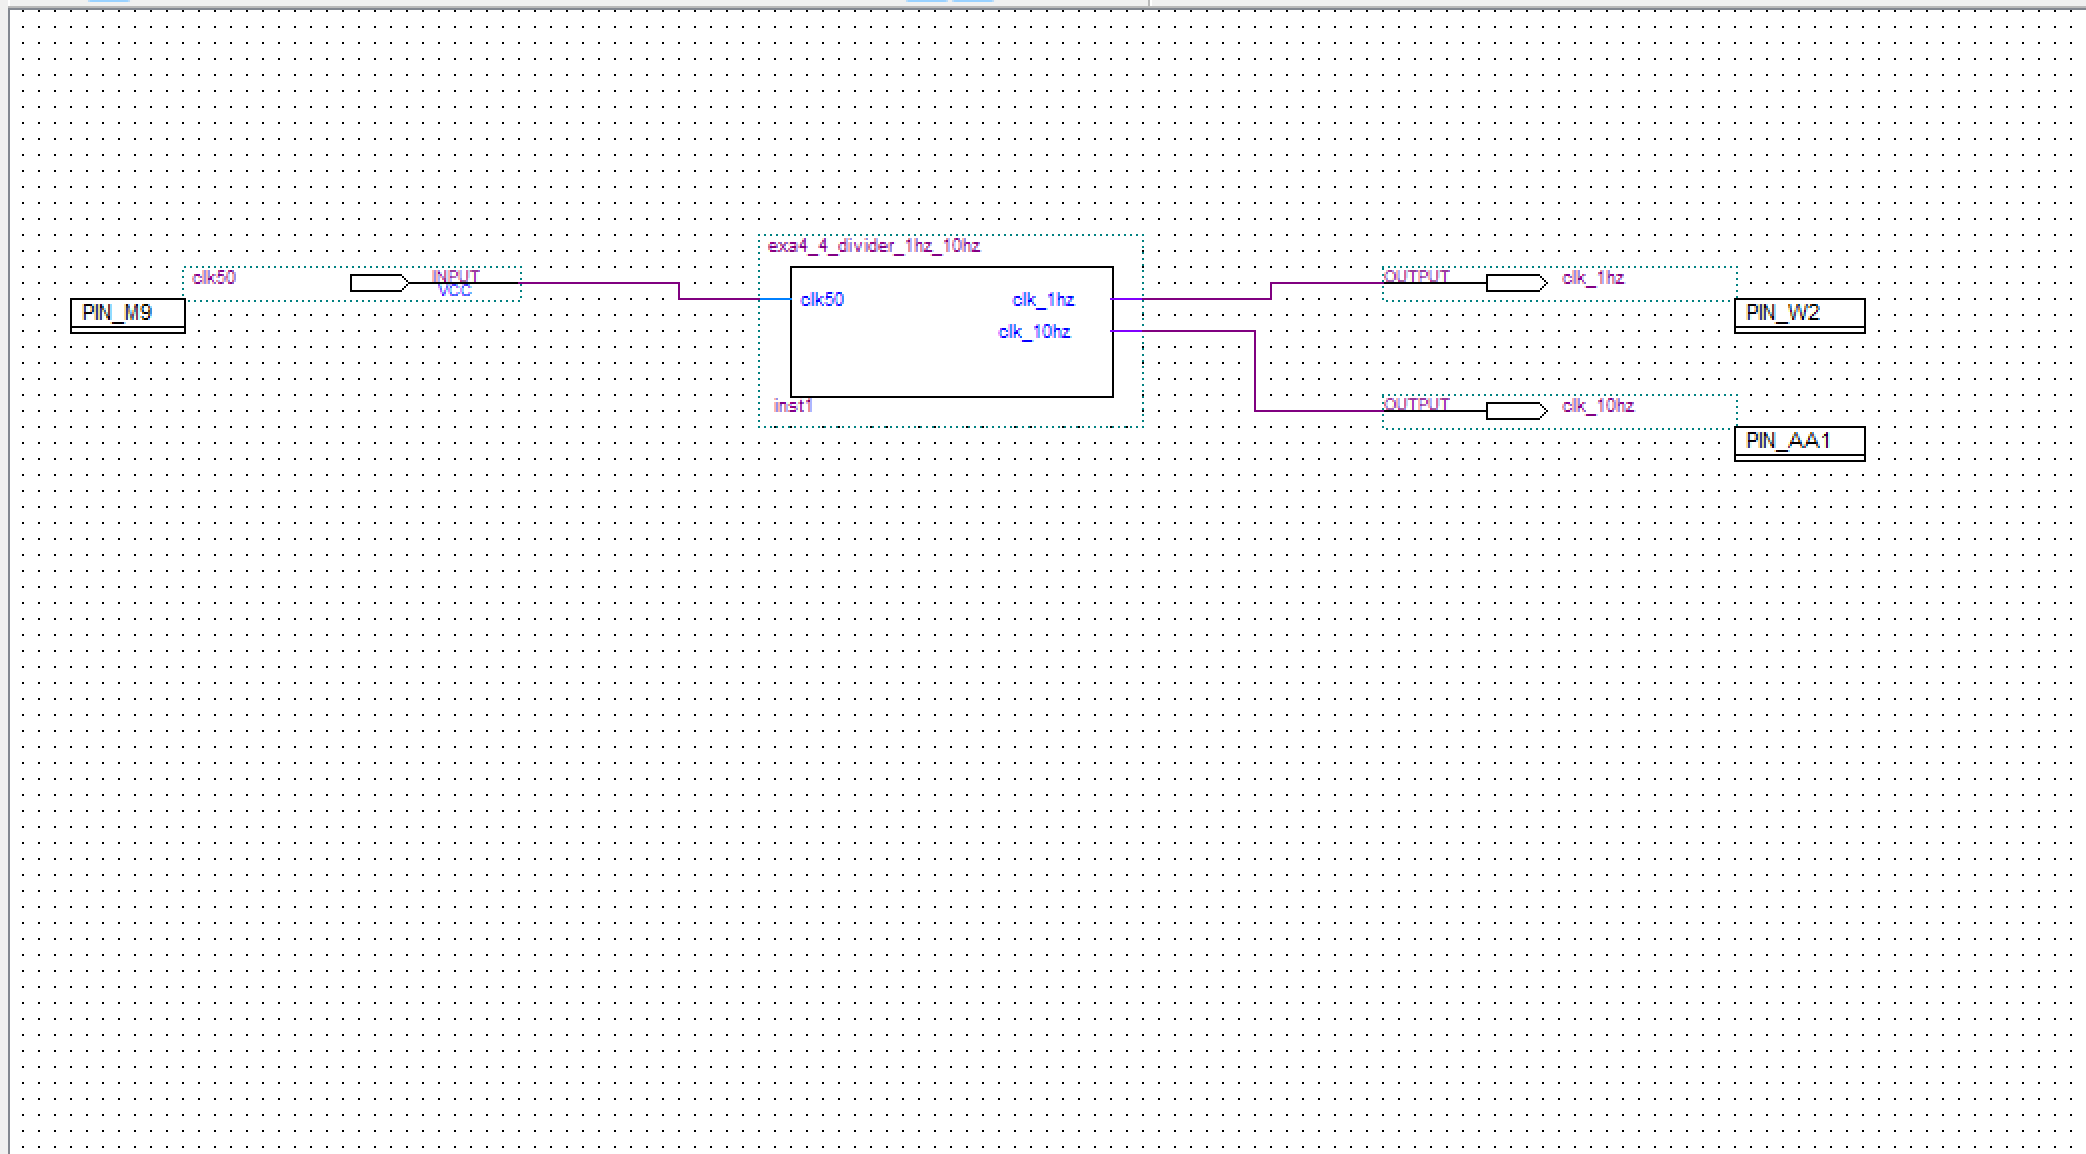
\includegraphics[width=0.85\textwidth]{要求4电路.png}
    \caption{要求 4 分频器 BDF 原理图}
    \label{fig:task4_circuit}
\end{figure}

\subsubsection{仿真验证与下载验证}

由于使用实际分频参数（25,000,000 和 2,500,000）进行波形仿真需要极长的仿真时间，可通过编写测试台文件，使用 \texttt{generic map} 将半周期参数缩小（如设为 4 和 2），在较短的仿真时间内验证分频逻辑的正确性。

引脚分配完成后重新编译并下载到 DE0 开发板。利用板上 50MHz 晶振作为输入时钟，观察 LEDR2 以 1 秒为周期闪烁（1Hz），LEDR1 以 0.1 秒为周期闪烁（10Hz），验证分频器功能正确。

\subsection{要求 5：综合设计}

\subsubsection{设计方案}

综合设计需要在一个七段数码管上循环显示 12 位字符 \texttt{2539FEEL3980}，并在每轮显示结束后自动切换 1Hz 和 10Hz 的显示速度。整个系统由三个核心 VHDL 模块和一个顶层 BDF 原理图组成。

\subsubsection{编写 VHDL 模块}

\paragraph{特殊七段码译码器（exa4\_2\_2）}

该译码器根据要求 5 的显示序列进行定制，将计数值 0--11 映射到对应的七段显示码。

\begin{minted}{vhdl}
-- 七段码译码器：显示 2539FEEL3980
library ieee;
use ieee.std_logic_1164.all;

entity exa4_2_2 is
port(
    BCD_IN : in  std_logic_vector(3 downto 0);
    SG_OUT : out std_logic_vector(6 downto 0)
);
end exa4_2_2;

architecture one of exa4_2_2 is
begin
process(BCD_IN)
begin
    case BCD_IN is
        when "0000" => SG_OUT <= "0100100"; -- 2
        when "0001" => SG_OUT <= "0010010"; -- 5
        when "0010" => SG_OUT <= "0110000"; -- 3
        when "0011" => SG_OUT <= "0010000"; -- 9
        when "0100" => SG_OUT <= "0001110"; -- F
        when "0101" => SG_OUT <= "0000110"; -- E
        when "0110" => SG_OUT <= "0000110"; -- E
        when "0111" => SG_OUT <= "1000111"; -- L
        when "1000" => SG_OUT <= "0110000"; -- 3
        when "1001" => SG_OUT <= "0010000"; -- 9
        when "1010" => SG_OUT <= "0000000"; -- 8
        when "1011" => SG_OUT <= "1000000"; -- 0
        when others => SG_OUT <= "1111111";
    end case;
end process;
end one;
\end{minted}
\captionof{listing}{特殊七段码译码器（exa4\_2\_2.vhd）}
\label{lst:decoder2}

\paragraph{M12 计数器（exa4\_3\_2）}

M12 计数器在模 15 计数器基础上修改为 0--11 循环，并新增使能信号 \texttt{en}，仅在使能有效时计数。

\begin{minted}{vhdl}
-- M12计数器：0~11循环，用于显示 2539FEEL3980 共12位
library ieee;
use ieee.std_logic_1164.all;
use ieee.numeric_std.all;

entity exa4_3_2 is
port(
    clk  : in  std_logic;
    rst  : in  std_logic;
    en   : in  std_logic;
    dout : out std_logic_vector(3 downto 0);
    cout : out std_logic
);
end exa4_3_2;

architecture one of exa4_3_2 is
signal Q1 : unsigned(3 downto 0) := (others => '0');
begin

process(clk, rst)
begin
    if rst = '0' then
        Q1 <= (others => '0');
        cout <= '0';

    elsif rising_edge(clk) then
        cout <= '0';

        if en = '1' then
            if Q1 = to_unsigned(11, 4) then
                Q1 <= (others => '0');
                cout <= '1';
            else
                Q1 <= Q1 + 1;
            end if;
        end if;
    end if;
end process;

dout <= std_logic_vector(Q1);

end one;
\end{minted}
\captionof{listing}{M12 计数器（exa4\_3\_2.vhd）}
\label{lst:counter2}

\paragraph{自动 1Hz/10Hz 切换控制器（exa4\_auto\_1hz\_10hz）}

该模块集成了分频和速度切换功能。内部维护一个模式标志 \texttt{mode}（0 表示 1Hz，1 表示 10Hz），每当收到 M12 计数器的 \texttt{loop\_end} 信号时切换模式。根据当前模式选择不同的分频系数，产生对应频率的 \texttt{tick} 脉冲。

\begin{minted}{vhdl}
-- 1Hz / 10Hz 自动切换tick发生器
library ieee;
use ieee.std_logic_1164.all;

entity exa4_auto_1hz_10hz is
port(
    clk50     : in  std_logic;
    rst       : in  std_logic;
    loop_end  : in  std_logic;
    tick      : out std_logic;
    speed_sel : out std_logic
);
end exa4_auto_1hz_10hz;

architecture rtl of exa4_auto_1hz_10hz is

constant DIV_1HZ  : integer := 50000000;
constant DIV_10HZ : integer := 5000000;

signal cnt    : integer range 0 to DIV_1HZ - 1 := 0;
signal mode   : std_logic := '0';
signal tick_r : std_logic := '0';

begin

process(clk50, rst)
    variable limit_v : integer;
begin
    if rst = '0' then
        cnt    <= 0;
        mode   <= '0';
        tick_r <= '0';

    elsif rising_edge(clk50) then
        tick_r <= '0';

        if loop_end = '1' then
            mode <= not mode;
            cnt  <= 0;

        else
            if mode = '0' then
                limit_v := DIV_1HZ - 1;
            else
                limit_v := DIV_10HZ - 1;
            end if;

            if cnt >= limit_v then
                cnt    <= 0;
                tick_r <= '1';
            else
                cnt <= cnt + 1;
            end if;
        end if;
    end if;
end process;

tick <= tick_r;
speed_sel <= mode;

end rtl;
\end{minted}
\captionof{listing}{自动 1Hz/10Hz 切换控制器（exa4\_auto\_1hz\_10hz.vhd）}
\label{lst:auto}

\subsubsection{生成原理图框图}

对上述三个 VHDL 模块分别进行编译，然后通过 \textbf{File $\rightarrow$ Create/Update $\rightarrow$ Create Symbol Files for Current File} 生成各自的 \texttt{.bsf} 模块符号文件，使其可在顶层原理图中作为元件调用。

\subsubsection{建立顶层原理图与引脚分配}

新建 BDF 原理图文件作为顶层设计，从 Project 元件库中依次放置三个模块符号，按照以下连接关系完成布线：

\begin{itemize}
    \item 50MHz 时钟（PIN\_M9）同时连接到 \texttt{exa4\_auto\_1hz\_10hz} 的 \texttt{clk50} 端和 \texttt{exa4\_3\_2} 的 \texttt{clk} 端。
    \item 复位信号（PIN\_U13，按键 SW0）同时连接到两个模块的 \texttt{rst} 端。
    \item \texttt{exa4\_auto\_1hz\_10hz} 的 \texttt{tick} 输出连接到 \texttt{exa4\_3\_2} 的 \texttt{en} 输入。
    \item \texttt{exa4\_3\_2} 的 \texttt{dout[3:0]} 连接到 \texttt{exa4\_2\_2} 的 \texttt{BCD\_IN[3:0]}。
    \item \texttt{exa4\_3\_2} 的 \texttt{cout} 反馈连接到 \texttt{exa4\_auto\_1hz\_10hz} 的 \texttt{loop\_end} 输入。
    \item \texttt{exa4\_2\_2} 的 \texttt{SG\_OUT[6:0]} 连接到 HEX0 数码管输出引脚。
\end{itemize}

引脚分配如表~\ref{tab:task5_pins} 所示，顶层原理图如图~\ref{fig:task5_circuit} 所示。

\begin{table}[H]
    \centering
    \caption{要求 5 引脚分配表}
    \label{tab:task5_pins}
    \begin{tabular}{ccc}
        \toprule
        \textbf{端口名} & \textbf{引脚} & \textbf{对应硬件} \\
        \midrule
        clk50 (pin\_name4) & PIN\_M9  & 50MHz 时钟 \\
        rst (pin\_name5)   & PIN\_U13 & SW0 \\
        SG\_OUT[6]         & PIN\_AA22 & HEX0[6] \\
        SG\_OUT[5]         & PIN\_Y21  & HEX0[5] \\
        SG\_OUT[4]         & PIN\_Y22  & HEX0[4] \\
        SG\_OUT[3]         & PIN\_W21  & HEX0[3] \\
        SG\_OUT[2]         & PIN\_W22  & HEX0[2] \\
        SG\_OUT[1]         & PIN\_V21  & HEX0[1] \\
        SG\_OUT[0]         & PIN\_U21  & HEX0[0] \\
        \bottomrule
    \end{tabular}
\end{table}

\begin{figure}[H]
    \centering
    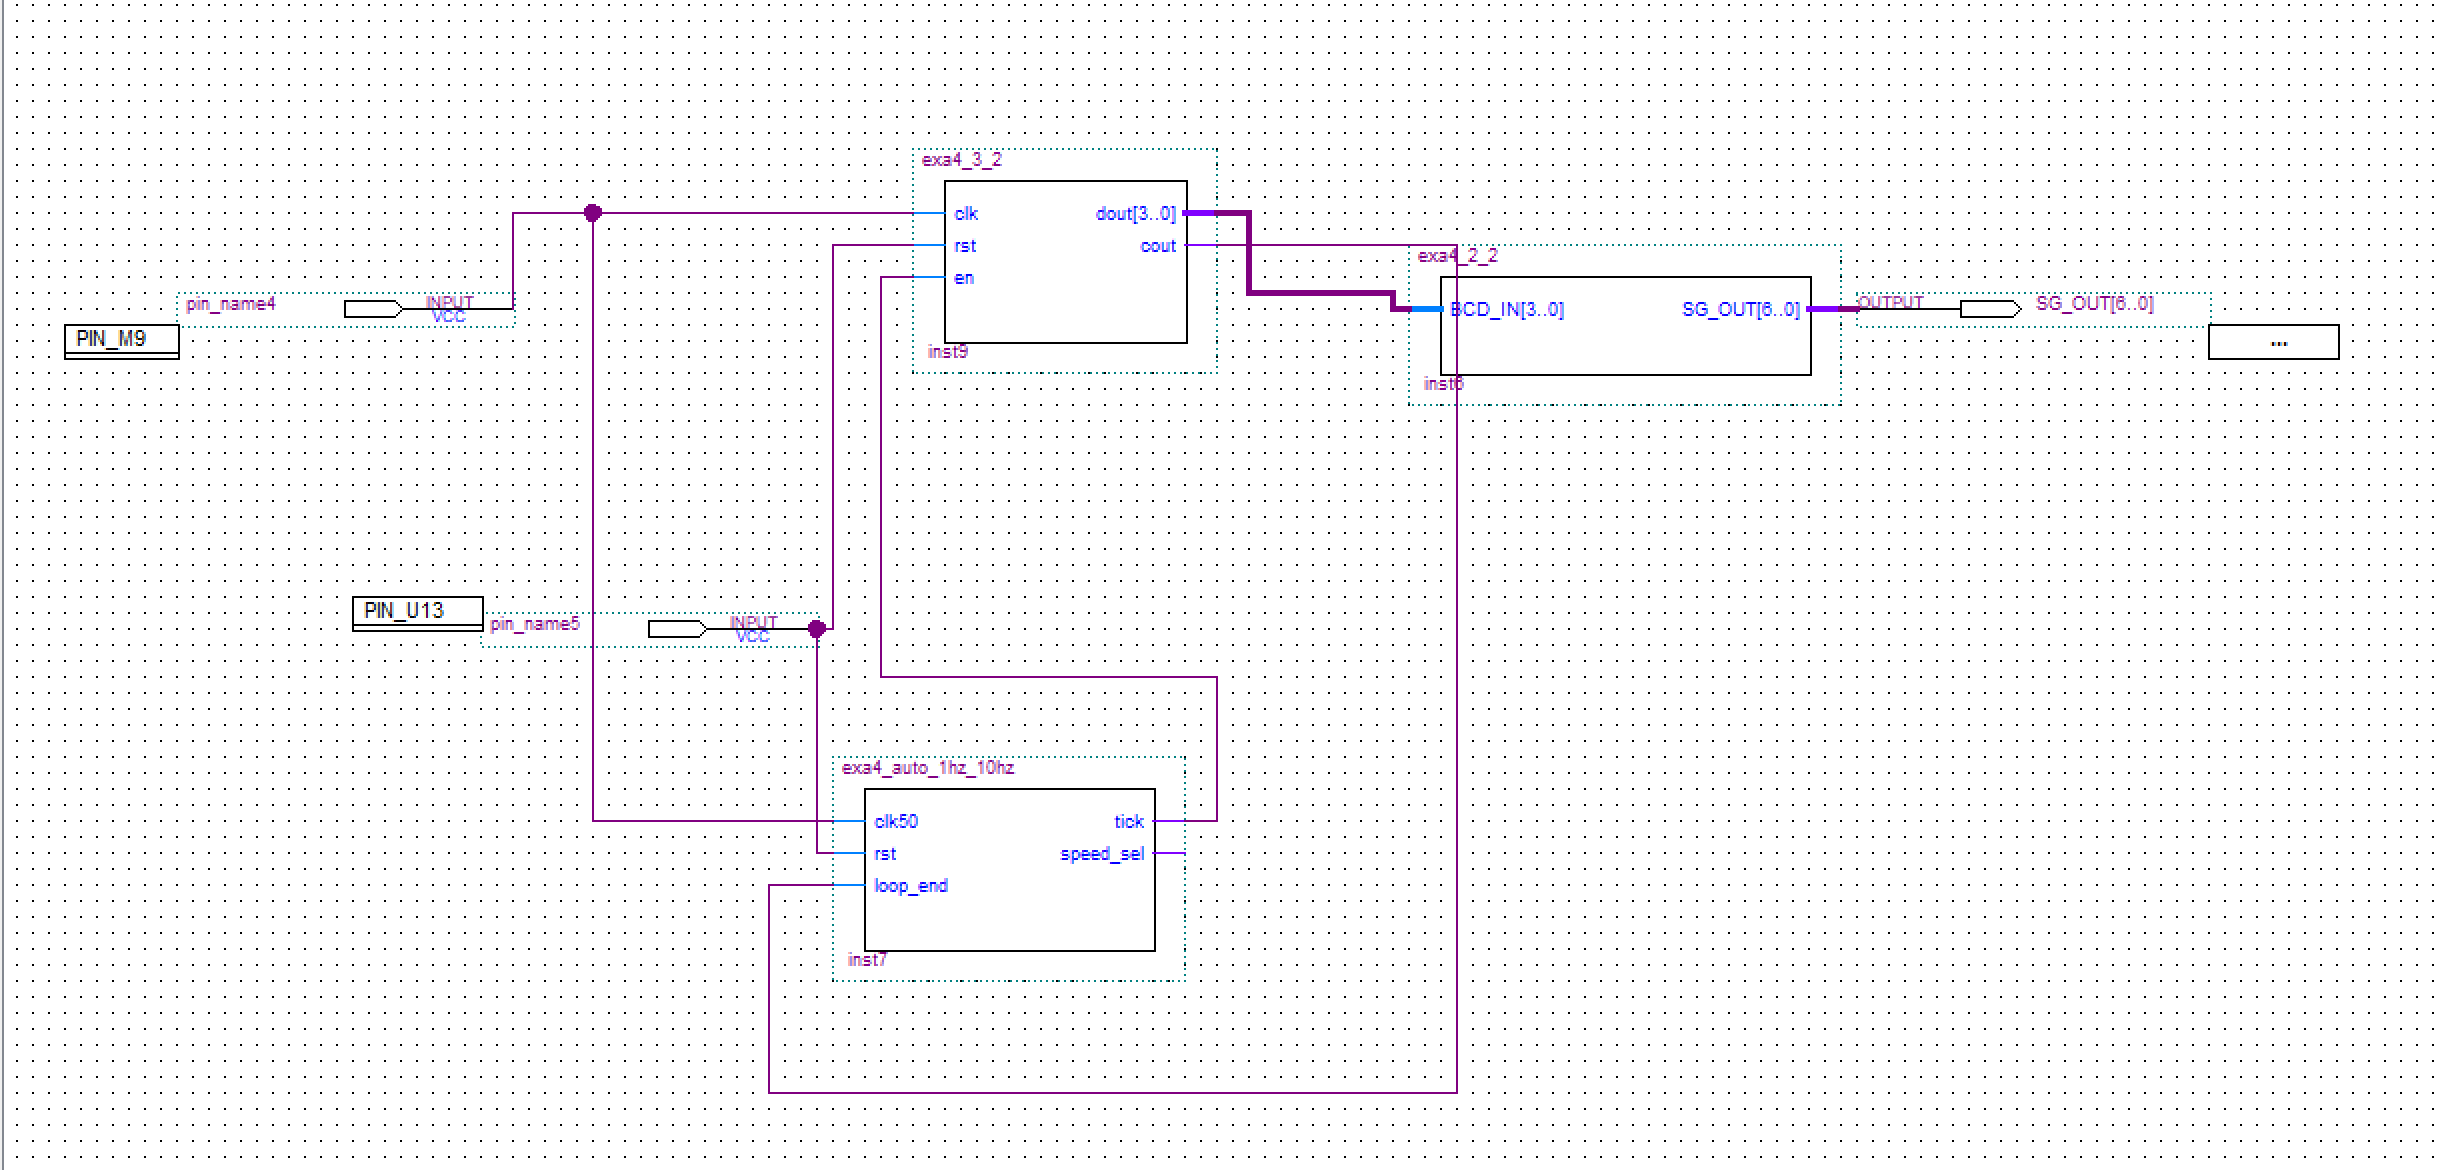
\includegraphics[width=0.95\textwidth]{要求5电路.png}
    \caption{要求 5 综合设计 BDF 原理图}
    \label{fig:task5_circuit}
\end{figure}

\subsubsection{编译与下载验证}

将 BDF 原理图文件设置为顶层实体，进行完整编译。确认编译无错误后，通过 USB-Blaster 以 JTAG 模式下载到 DE0 开发板。

下载完成后，观察 HEX0 数码管的显示行为：数码管以 1Hz 的速度依次显示 2, 5, 3, 9, F, E, E, L, 3, 9, 8, 0 共 12 个字符，完成一轮后自动切换到 10Hz 速度进行下一轮循环显示，然后再切回 1Hz，如此交替进行。按下复位键可使显示从第一个字符重新开始。

\section{实验过程中的问题}

\begin{enumerate}
    \item \textbf{VHDL 模块生成原理图框图}：本实验首次使用 VHDL 描述电路模块。初次操作时不清楚如何将 VHDL 文件变为可在 BDF 原理图中调用的元件。关键步骤是编译 VHDL 文件后，选择 File $\rightarrow$ Create/Update $\rightarrow$ Create Symbol Files for Current File 生成 \texttt{.bsf} 符号文件。若跳过此步骤，在元件库中将找不到对应模块。
    \item \textbf{分频器仿真时间过长}：使用实际半周期参数（25,000,000）进行波形仿真时，即使只观察一个完整周期也需要模拟 5000 万个时钟周期，仿真耗时极长。解决方法是编写测试台文件，通过 \texttt{generic map} 将半周期参数缩小为较小的值（如 4 和 2），在合理的仿真时间内验证分频逻辑是否正确。
    \item \textbf{七段数码管有效电平}：DE0 开发板的七段数码管为共阳极结构，段选信号低电平有效（输出 0 点亮对应段，输出 1 熄灭对应段）。若译码器的段选编码极性错误，数码管上所有笔段会出现反转显示。本实验的 VHDL 代码中已按低电平有效编码，可直接驱动数码管。
    \item \textbf{综合设计中模块间的反馈连接}：要求 5 中，M12 计数器的 \texttt{cout} 输出需反馈到自动切换控制器的 \texttt{loop\_end} 输入，而控制器的 \texttt{tick} 输出又连接到计数器的 \texttt{en} 输入，形成闭环。若任一反馈连线缺失，系统将无法正常工作：缺少 \texttt{tick} 连接时计数器不会计数，缺少 \texttt{cout} 反馈时速度无法切换。
\end{enumerate}

\section{心得体会}

\begin{enumerate}
    \item 通过本次实验，我初步掌握了 VHDL 硬件描述语言的基本语法和设计方法。与前几次实验中使用的原理图输入方式相比，VHDL 能够用简洁的文字代码描述复杂的逻辑功能，尤其在实现译码器、计数器等功能模块时，代码方式比手工连线更加高效且不易出错。
    \item 本实验从简单的异或门出发，逐步过渡到译码器、计数器、分频器，最终完成多模块综合设计，让我深刻体会到模块化设计的思想。每个功能模块可以独立设计、独立仿真验证，确认正确后再在顶层进行集成，大大降低了复杂系统的调试难度。
    \item 要求 5 的综合设计将 VHDL 文本描述与 BDF 图形化连接相结合，发挥了两种设计方法各自的优势：VHDL 适合描述功能逻辑，BDF 原理图适合展示模块间的连接关系和信号流向。这种混合设计方法在实际的 FPGA 工程开发中也是常用的实践方式。
\end{enumerate}

\end{document}
